\chapter{Testy i porównanie algorytmów}
\section{Analiza działania poszczególnych algorytmów}
\subsection{Algorytm Roju Cząsteczek}
\subsubsection{Problem z proponowanym rozwiązaniem}
\par Podczas testowania proponowanego rozwiązania wystąpił problem. Algorytm wykazał się słabą skutecznością i nie był w stanie usunąć całkowicie problemów związanych z twadrymi ograniczeniami. Jak wiemy z rozdziału drugiego ograniczania te w ostatecznym rozwiązaniu nie mają prawa być łamane.
\par Aby algorytm brał pod uwagę w pierwszej kolejności twarde ograniczenia, naruszenie każdego z tych ograniczeń związane jest z przydzieleniem dodatkowej kary pomnożonej przez milion.
Poniższy wykres pokazuje efektywność algorytmu. Uwagę należy zwrócić na skalę przyjętą na osi y. Wartości nie schodzą poniżej $10^{7}$ czyli wynik w najlepszym wypadku nadal łamie 10 twardych ograniczeń.
\begin{figure}[H]
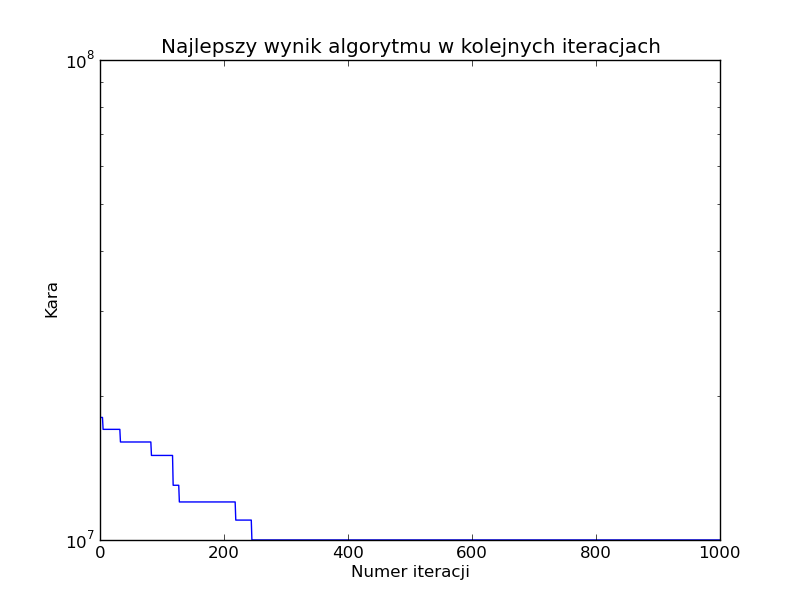
\includegraphics[width=10cm]{img/standard_penalty.png}
\centering
\end{figure}
\par W celu sprawdzenia przyczyny tego zachowania przyjrzałem się zachowaniu pojedynczej cząsteczki. Okazało się, że kara za kolejno generowane plany oscyluje wokół kary wyliczonej dla początkowego planu, co potwierdza poniższy wykres.  
\begin{figure}[H]
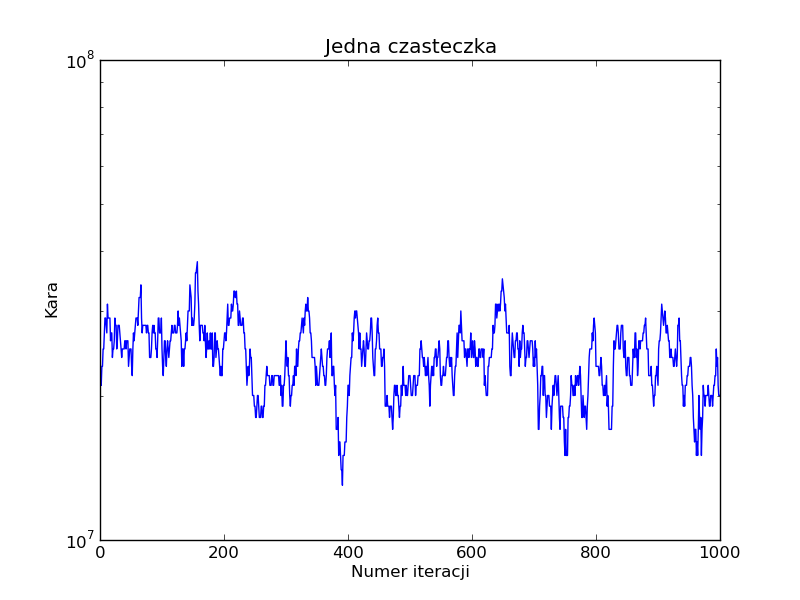
\includegraphics[width=10cm]{img/standard_particle.png}
\centering
\end{figure}
\par Na podstawie dalszej analizy okazało się, że wszystkie cząsteczki zachowują się bardzo podobnie. Widać to na poniższym wykresie.
\begin{figure}[H]
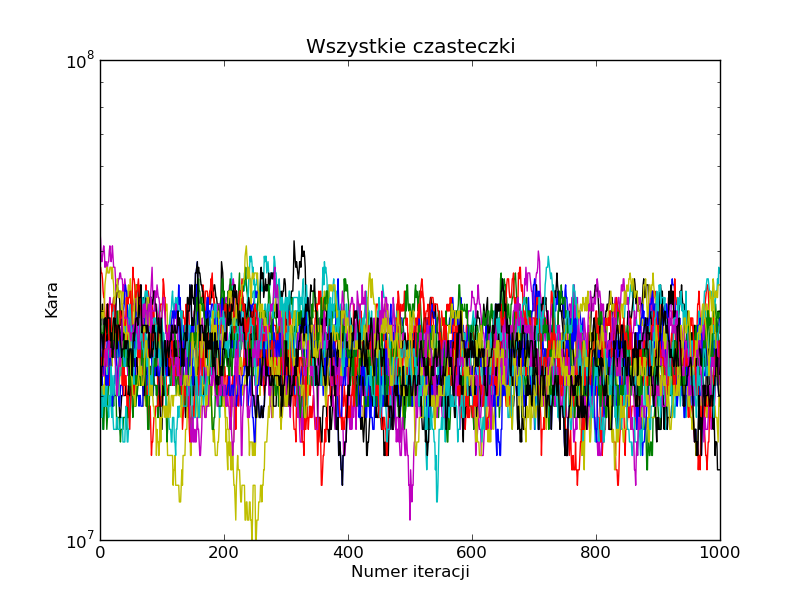
\includegraphics[width=10cm]{img/standard_particle_all.png}
\centering
\end{figure}
\subsubsection{Rozważane modyfikacje}
\par Rozważyłem dwie modyfikacje do aktualnego algorytmu. Jedną nazwałem podążaniem za lokalnie najlepszym planem, a drugą podążanie za globalnie najlepszym planem. Obie modyfikacje są względem siebie analogiczne, a różnią się tylko tym który plan bierzemy pod uwagę. Modyfikacją została objęta faza oceny aktualnego rozwiązania, która zachodzi na początku każdej iteracji. Dodany został warunek, że jeśli aktualny plan jest gorszy od najlepszego planu to zostaje on zamieniony na najlepszy plan. Usunięte też zostały kroki 3 i 4 czyli kopie z najlepszych planów.
\par W przypadku gdy każda cząsteczka podąża za swoim lokalnie najlepszym planem istnieje mniejsze ryzyko, że algorytm utknie w minimum lokalnym przestrzeni rozwiązań. Natomiast podczas podążania za globalnie najlepszym planem algorytm będzie znacznie szybciej dążył do najbliższego minimum.
\par Opcja podążania za lokalnie najlepszym planem okazała się być dużo efektywniejsza od podstawowego algorytmu. W tym przypadku twarde ograniczenia nie stanowiły problemu. Można to zobaczyć na poniższym wykresie.
\begin{figure}[H]
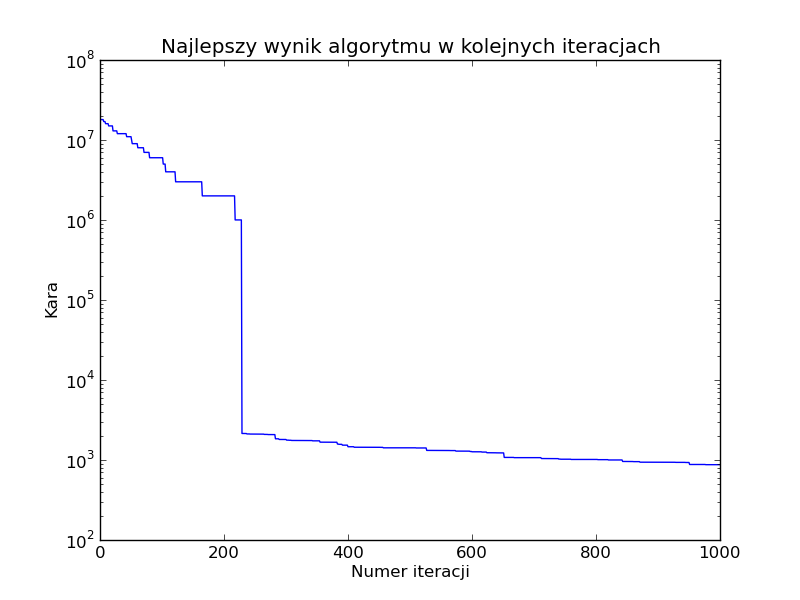
\includegraphics[width=10cm]{img/localbest_penalty.png}
\centering
\end{figure}
\par Analizując pojedynczą cząsteczkę można zauważyć, że często kara waha się od małych wartości do wartości milionowych. Jest to spowodowane tym, że w po zamianie dwóch lekcji w poprzedniej iteracji pojawił się konflikt z twardymi ograniczeniami. Nie stanowi to problemu, ponieważ w takim przypadku wracamy do poprzedniego rozwiązania. Na poniższych wykresach widać zachowanie dla pojedynczej cząsteczki oraz dla wszystkich cząsteczek.
\begin{figure}[H]
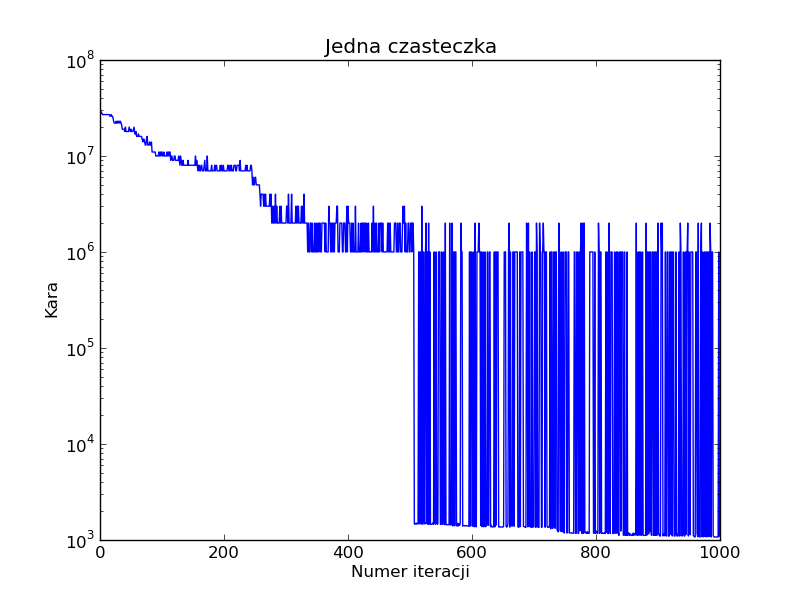
\includegraphics[width=10cm]{img/localbest_particle.png}
\centering
\end{figure}
\begin{figure}[H]
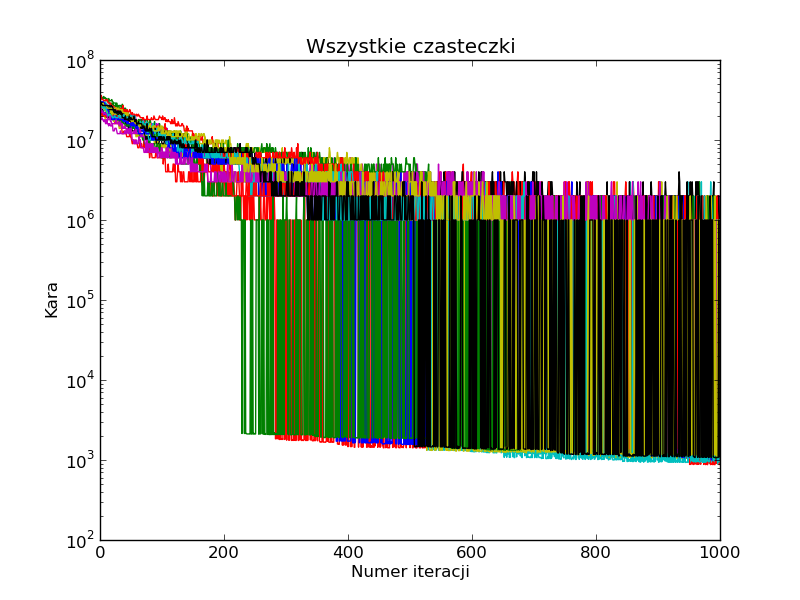
\includegraphics[width=10cm]{img/localbest_particle_all.png}
\centering
\end{figure}
\par Opcja podążania za globalnie najlepszym planem okazała się jeszcze bardziej efektywna. Sporym zaskoczeniem był brak problemów z lokalnymi minimami przestrzeni rozwiązań. Poniższy wykres pokazuje skuteczność modyfikacji.
\begin{figure}[H]
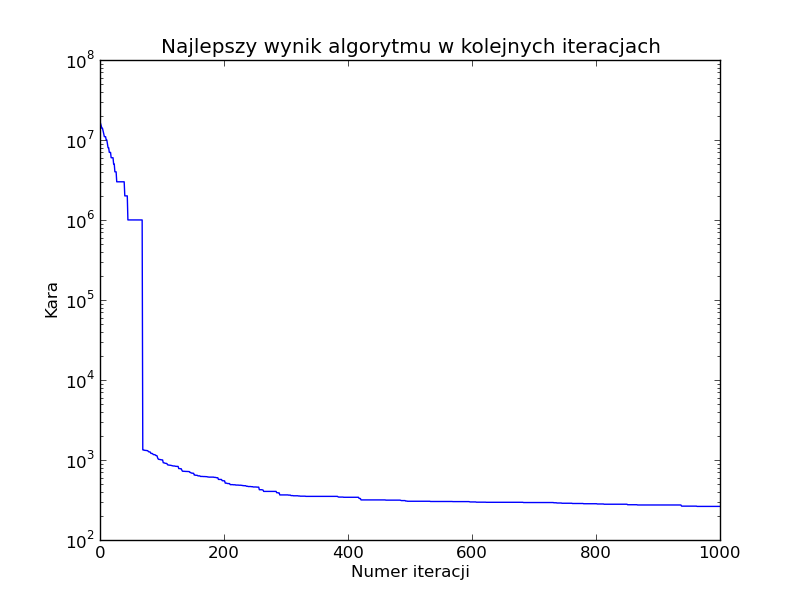
\includegraphics[width=10cm]{img/globalbest_penalty.png}
\centering
\end{figure}
\par W tym przypadku cząsteczki zachowywały się bardzo podobnie. Jedyną różnicą była prędkość z jaką spadała kara. Widać to na poniższych wykresach. 
\begin{figure}[H]
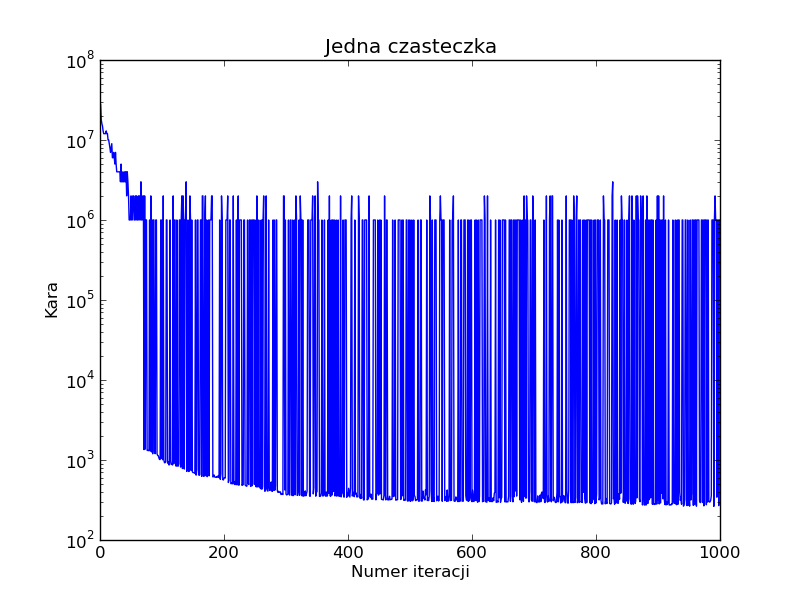
\includegraphics[width=10cm]{img/globalbest_particle.png}
\centering
\end{figure}
\begin{figure}[H]
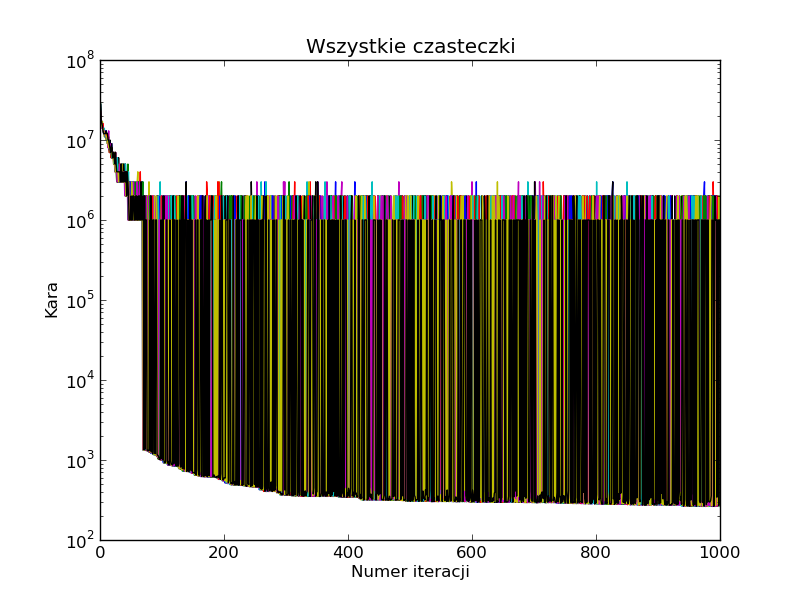
\includegraphics[width=10cm]{img/globalbest_particle_all.png}
\centering
\end{figure}
\subsubsection{Ostateczne rozwiązanie}
\par Jako ostateczne rozwiązanie wybrałem podążanie za globalnie najlepszym planem. Jest to spowodowane tym, że mimo wielu testów nie udało mi się znaleźć przypadku kiedy podążanie za lokalnie najlepszym planem wypadłoby lepiej. 
\subsection{Algorytm Adaptacyjny Tabu}
Przedstawienie działania algorytmu dla wybranych testów.
\par \textbf{Test 1}
\begin{figure}[H]
  \caption{Wykres zależności funkcji oceny od czasu}
  \centering
    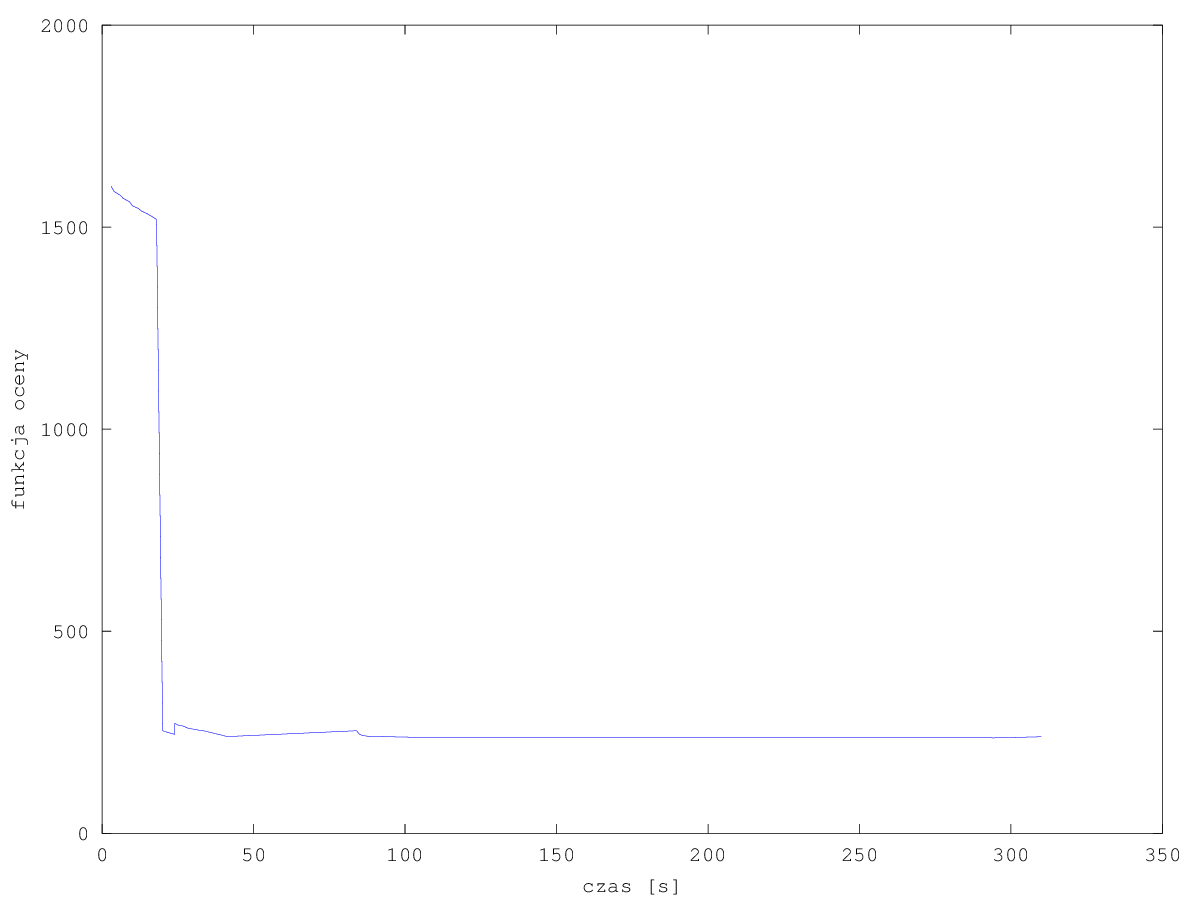
\includegraphics[width=0.8\textwidth]{ogolny.png}
\end{figure}
\begin{figure}[H]
  \caption{Wykres zależności funkcji oceny od czasu, bez uwzględnienia fazy inicjalizacji}
  \centering
    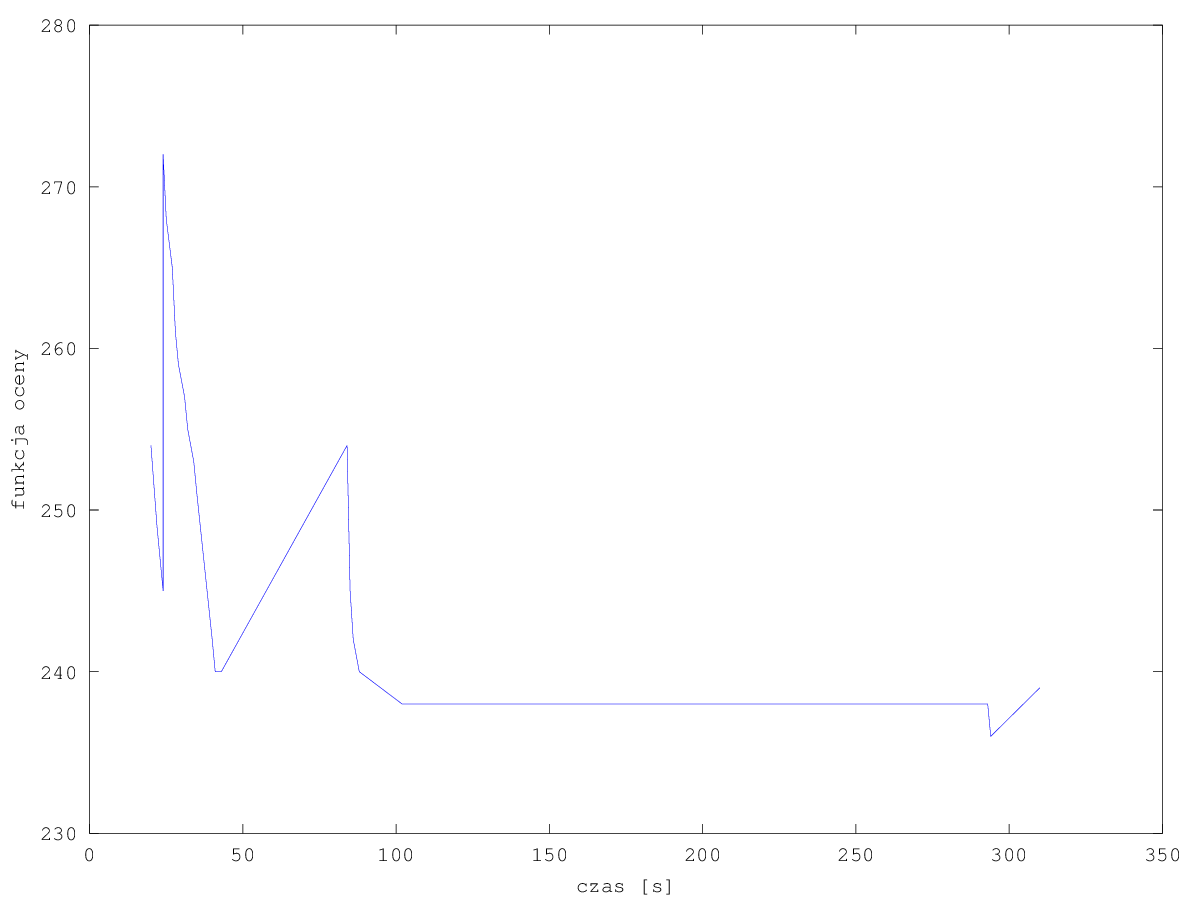
\includegraphics[width=0.8\textwidth]{szczeg.png}
\end{figure}
\par \textbf{Test 2}
\begin{figure}[H]
  \caption{Wykres zależności funkcji oceny od czasu}
  \centering
    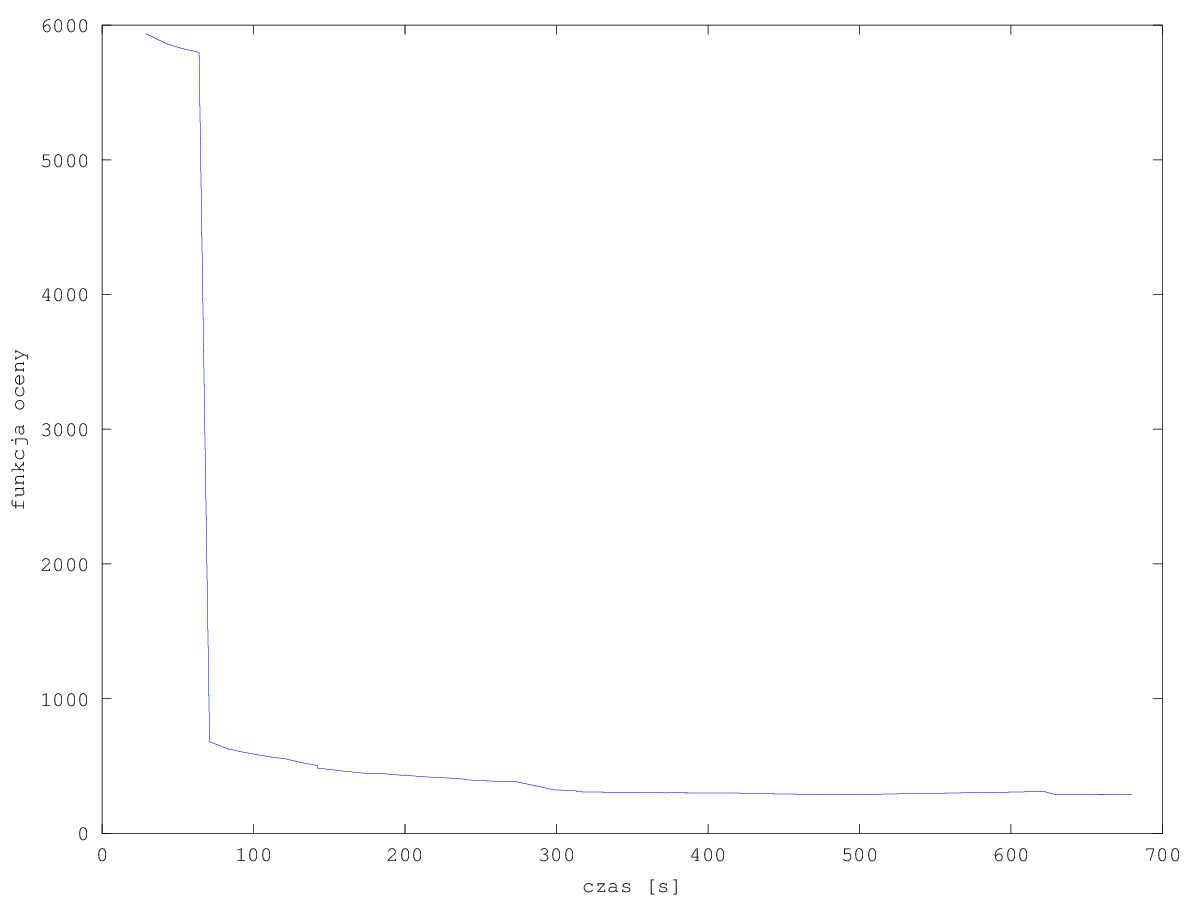
\includegraphics[width=0.8\textwidth]{ogolny2_instancja.png}
\end{figure}
\begin{figure}[H]
  \caption{Wykres zależności funkcji oceny od czasu, bez uwzględnienia fazy inicjalizacji}
  \centering
    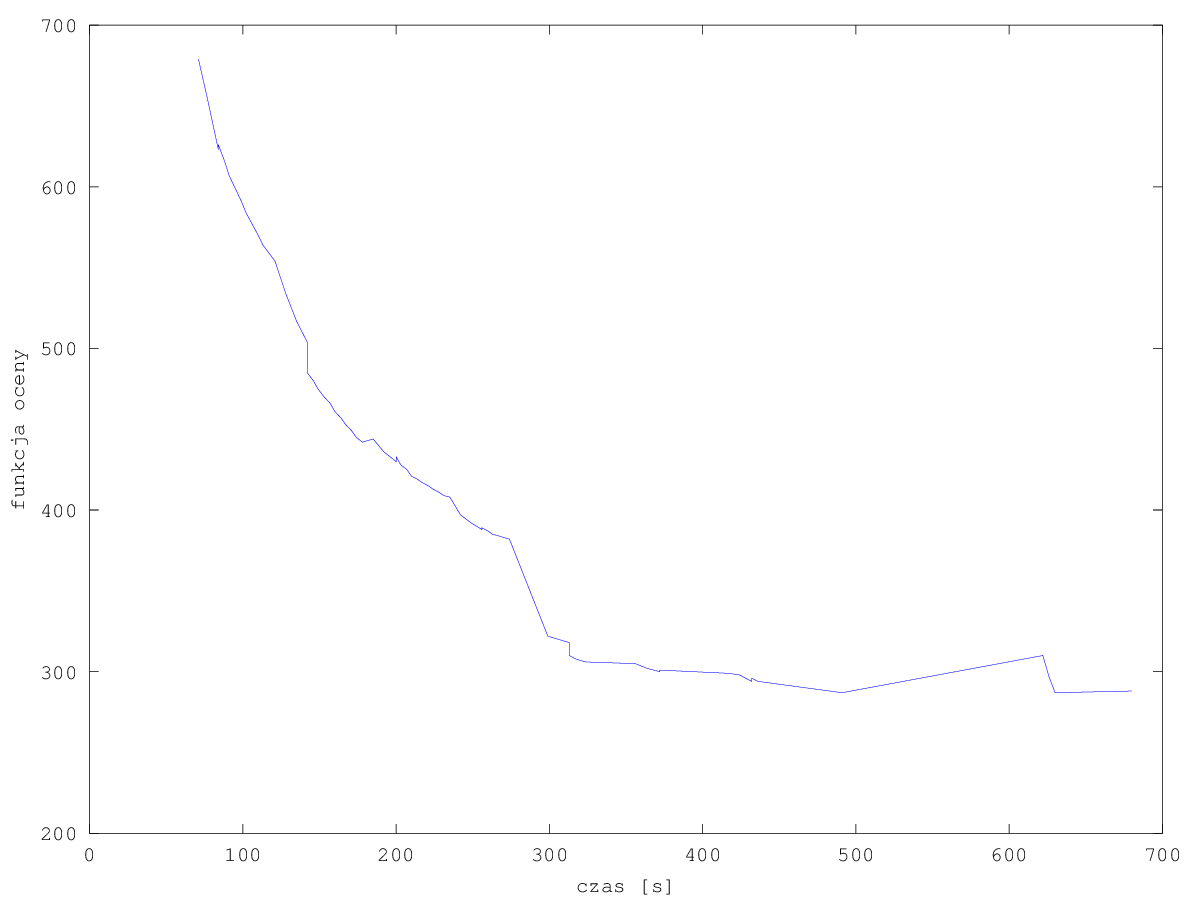
\includegraphics[width=0.8\textwidth]{szczegolowy2_instancja.png}
\end{figure}
\subsection{Algorytm Genetyczny}
\section{Specyfikacja testów}
Dane testowe pobrane zostały z konkursu ,,International Timetabling Competition 2007''
\subsection{Test 1}
\begin{table}[H]
\begin{center}

\begin{tabular}{ |c|c|c|c| }
\multicolumn{1}{r}{}
 &  \multicolumn{1}{c}{$$}
 & \multicolumn{1}{c}{$$} 
 \\
\cline{1-2}
$Liczba\ kursów$ & $30$\\
\cline{1-2}
$Liczba\ programów\ nauczania$ & $14$\\
\cline{1-2}
$Liczba\ dni$ & $5$ \\
\cline{1-2}
$Licza\ przedziałów\ czasowych$ & $6$ \\
\cline{1-2}
$Liczba\ ograniczeń$ & $53$ \\
\cline{1-2}
$Liczba\ sal$ & $6$ \\
\cline{1-2}
\end{tabular}
\end{center}
\caption {Specyfikacja danych - Test 1}
\end{table}
\subsubsection{Test 1 - wizualizacja}


\begin{figure}[H]
  \caption{Graf przedstawiający wszystkie zależności pomiędzy kursami (uwzględniając tych samych prowadzących nauczycieli oraz należenie kursu do tego samego programu nauczania) }
  \centering
    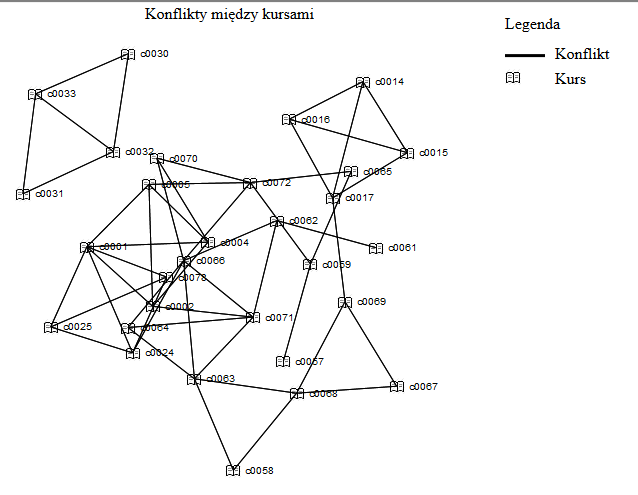
\includegraphics[width=0.8\textwidth]{test1.PNG}
\end{figure}


\begin{figure}[H]
  \caption{Graf uwzględniający zależności pomiędzy kursami uwzględniając prowadzących dane kursy}
  \centering
    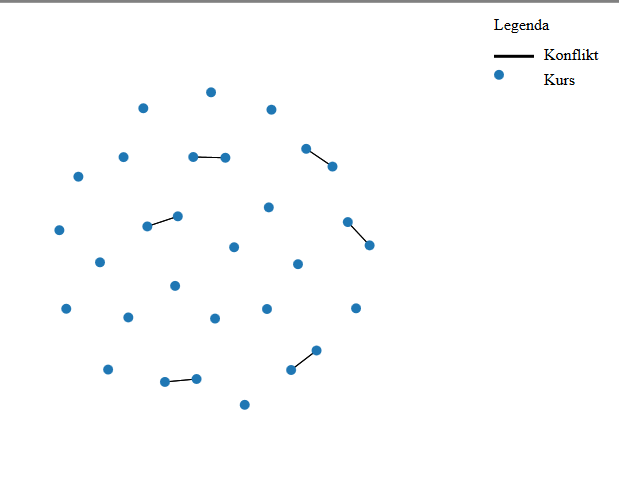
\includegraphics[width=0.8\textwidth]{test1_teach.PNG}
\end{figure}
\begin{figure}[H]
  \caption{Graf uwględniający grupy zależnych od siebie kursów wchodzących w skład tego samego programu nauczania}
  \centering
    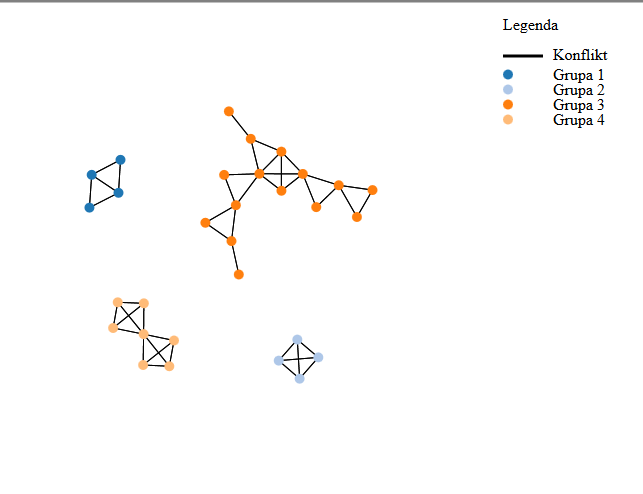
\includegraphics[width=0.8\textwidth]{test1_con.PNG}
\end{figure}
\subsection{Test 2}
\begin{table}[H]
\begin{center}

\begin{tabular}{ |c|c|c|c| }
\multicolumn{1}{r}{}
 &  \multicolumn{1}{c}{$$}
 & \multicolumn{1}{c}{$$} 
 \\
\cline{1-2}
$Liczba\ kursów$ & $82$\\
\cline{1-2}
$Liczba\ programów\ nauczania$ & $70$\\
\cline{1-2}
$Liczba\ dni$ & $5$ \\
\cline{1-2}
$Licza\ przedziałów\ czasowych$ & $5$ \\
\cline{1-2}
$Liczba\ ograniczeń$ & $513$ \\
\cline{1-2}
$Liczba\ sal$ & $16$ \\
\cline{1-2}
\end{tabular}
\end{center}
\caption {Specyfikacja danych - Test 2}
\end{table}
\subsection{Test 3}
\begin{table}[H]
\begin{center}

\begin{tabular}{ |c|c|c|c| }
\multicolumn{1}{r}{}
 &  \multicolumn{1}{c}{$$}
 & \multicolumn{1}{c}{$$} 
 \\
\cline{1-2}
$Liczba\ kursów$ & $72$\\
\cline{1-2}
$Liczba\ programów\ nauczania$ & $68$\\
\cline{1-2}
$Liczba\ dni$ & $5$ \\
\cline{1-2}
$Licza\ przedziałów\ czasowych$ & $5$ \\
\cline{1-2}
$Liczba\ ograniczeń$ & $382$ \\
\cline{1-2}
$Liczba\ sal$ & $16$ \\
\cline{1-2}
\end{tabular}
\end{center}
\caption {Specyfikacja danych - Test 3}
\end{table}






